\begin{figure}
  \begin{center}
    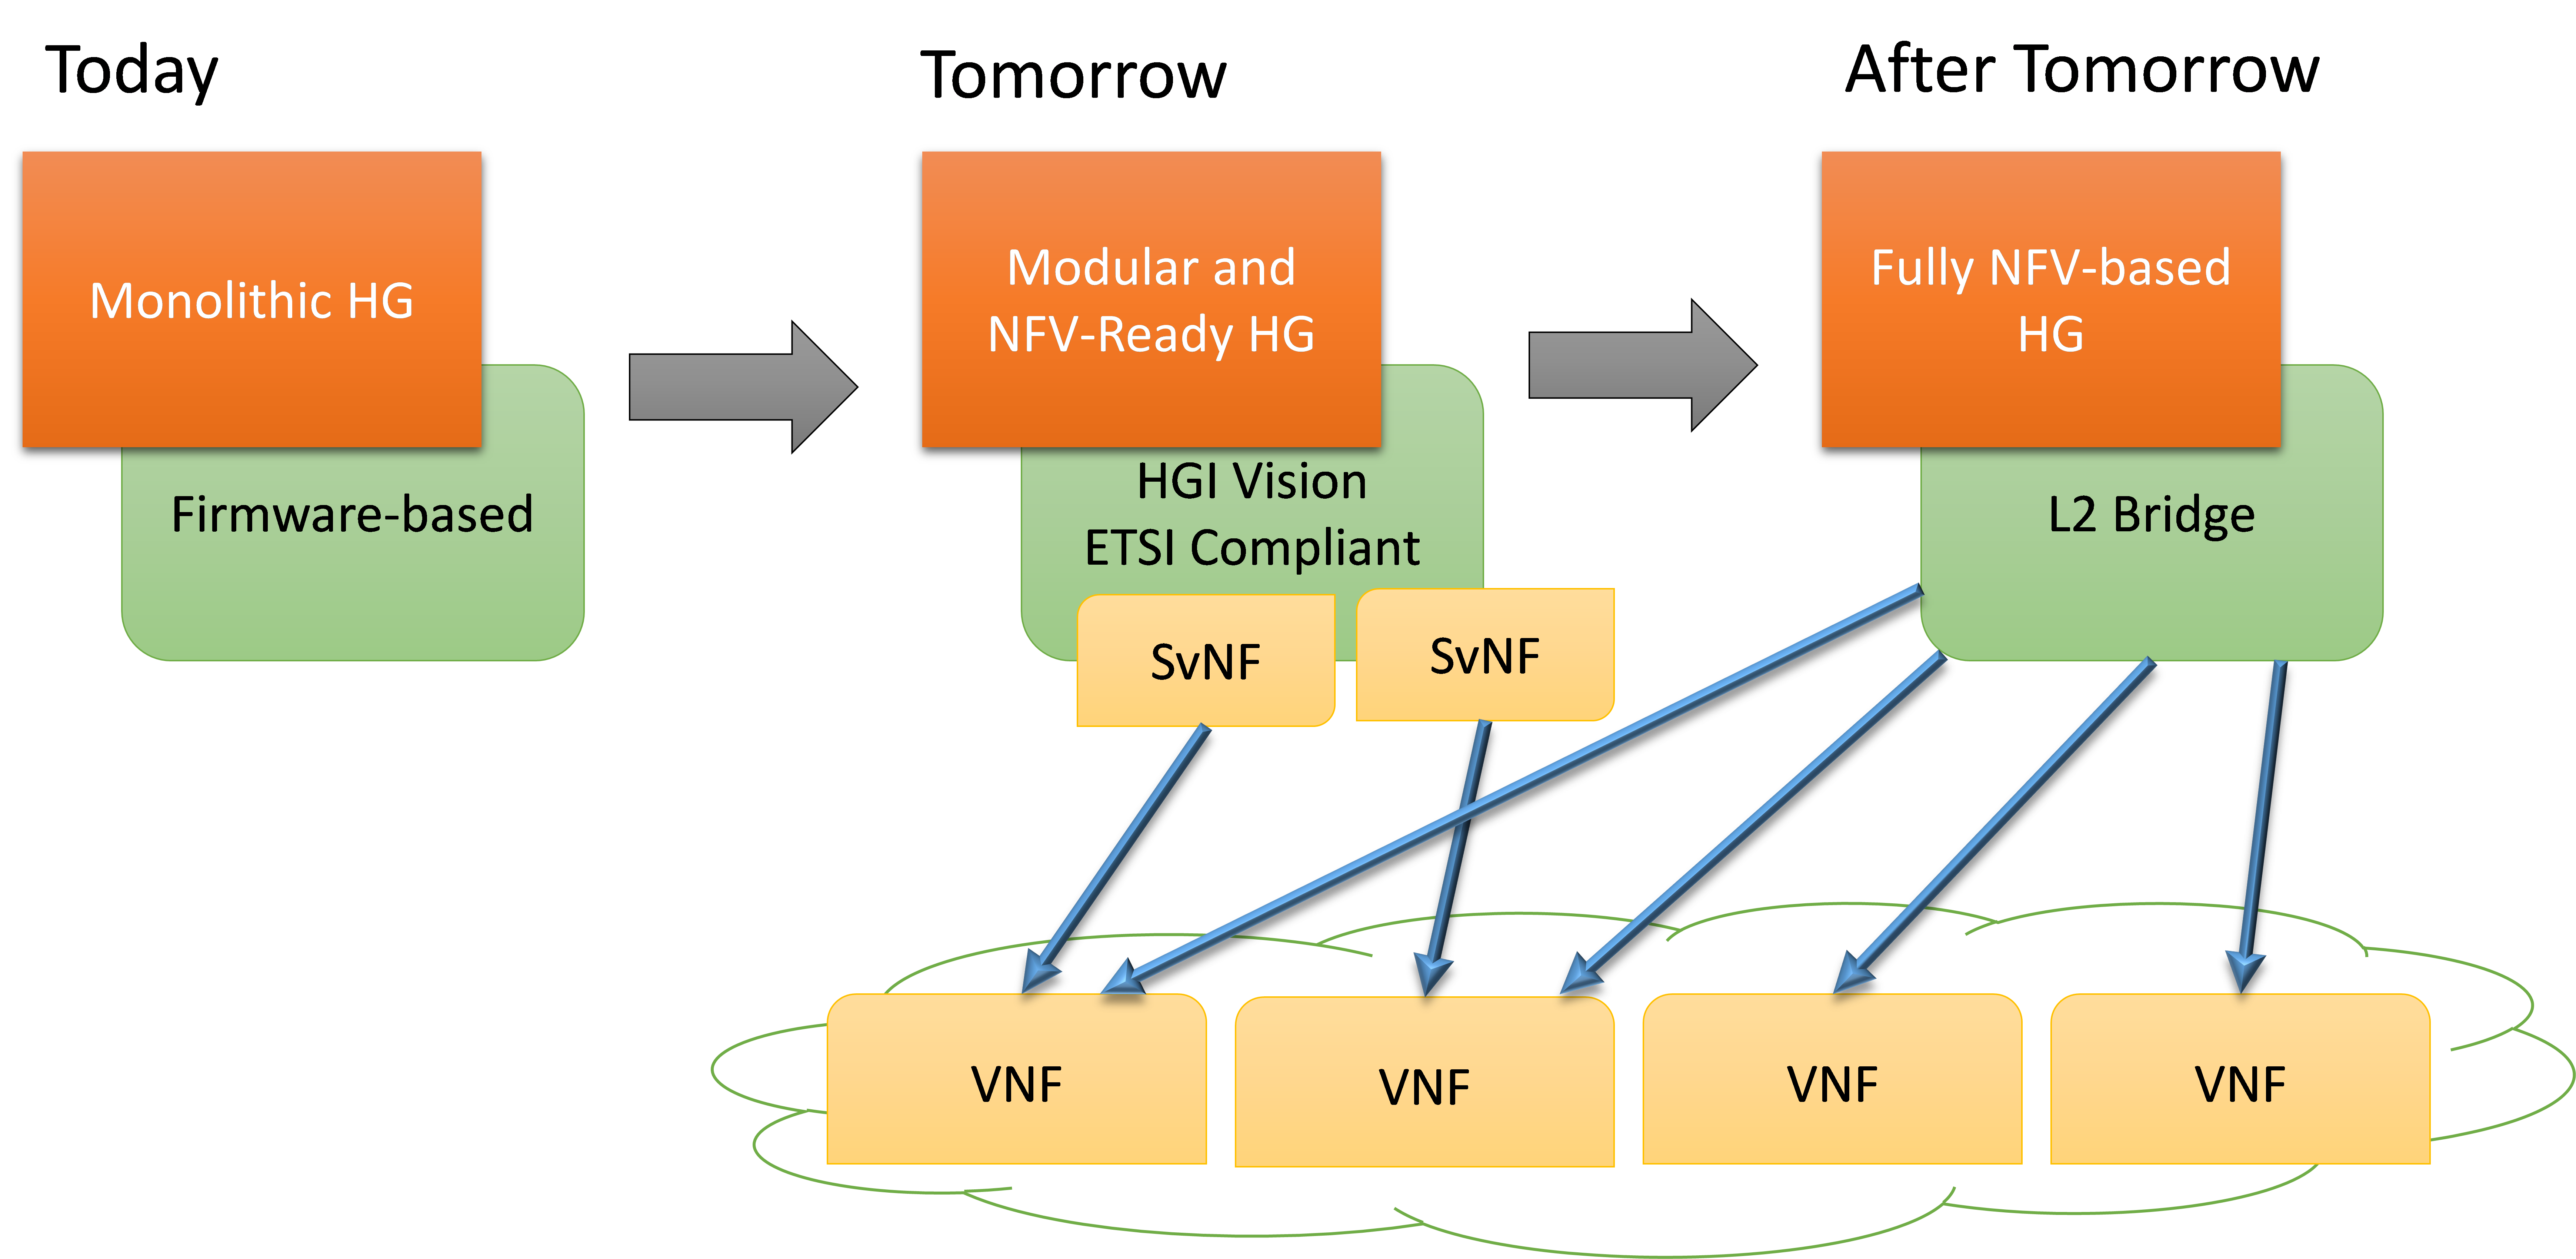
\includegraphics[width=0.45\textwidth,natwidth=6955,natheight=3398]{fig/vhgMigrationPath.png}
  \end{center}
  \caption{ Migration path from Modular to Virtual HG.
    \label{fig:migration}
  }
\end{figure}

Given all the advantages brought by the virtualization of the home environement, we should see a dramatic market swap.
Even if field studies are currently conducted\footnote{Telefónica and NEC win innovation award for virtualized home gateway trials: http://tinyurl.com/o8cl3bv}, they focus mainly on emerging markets.
For more mature markets, SPs balance those advantages with the necessity to dampen their past investments for their current infrastructure.
There is also a technological risk in building VHG infrastructure at scale, especially in a deflationary market where investments need to take opportunistic pathes. 

Focusing on the introduction of new services made possible by virtualization techniques has the advantage of not beeing too disturbing for the current infrastructure, while paving the way for a future migration to a full fledge virtual environment. Our proposal is to demonstrate that with the current infrastrusture, we can integrate NFV within the gateways to deploy new services easily.


\subsection{The NFV ready Modular HG}
We propose an alternative migration path where vNFs collaborate with modular gateways.
Figure~\ref{fig:migration} presents a Modular HG with \textit{"Surrogate vNF"} (SvNF) deployed on the device.
A SvNF is an OSGi bundle that acts like a regular module from the HG standpoint, except that it delegates any significant operation to a vNF.

To offer a proper support to OSGi SvNF modules can be aware of SP access network capabilities to support vNFs, so they can be registered in the HG OSGi execution environment only if they are supported by the underlying network.
For example, if the gateway cannot find any suitable vNF in a predefined SP point of presence (POP) list, it will fall back on legacy mode and keep using the native functionality instead of the virtualized one.

The key role played by the couple SvNF+vNF in the migration path is that the vNF part is used on both the OSGi modular gateway scenario and on the L2 bridge scenario.
This approach helps the SP stabilising its vNF before gradually migrating all its customers to the full vNF solution while securing investments made on developing the vNF.
 
\subsection{Concept and feasibility}
To demonstrate the feasibility of a modular and NFV-ready HG, we realized a proof of concept (POC).
In order for this POC to be highly relevant, we had to consider the best possible Network Functions to be virtualised.
We could have focused on core functions such as DHCP or NAT, which are challenging to virtualize at scale. However, virtualizing them doesn't illustrate how new services and features could be rolled out easily on the gateway.

We thus decided to highlight the advantages of our proposal by deploying a new type of SvNF+vNF related to video distribution that would leverage the End-User's Quality of Experience related to video consumption and enhance network performances at the same time.
Such a function can be introduced into a modular OSGi HG and its execution would definitely be efficient as a vNF, due to the heavy video processing tasks it involves.
It is expected that IP video traffic will reach almost 80\% of all consumer Internet traffic in 2018 \footnote{CISCO forecast white paper http://bit.ly/LVhmuL }, therefore it seems important to focus on how new solutions, such as NFV, could not only cope with this but especially enhance the delivery of such data.

\begin{figure*}
	
	\center

	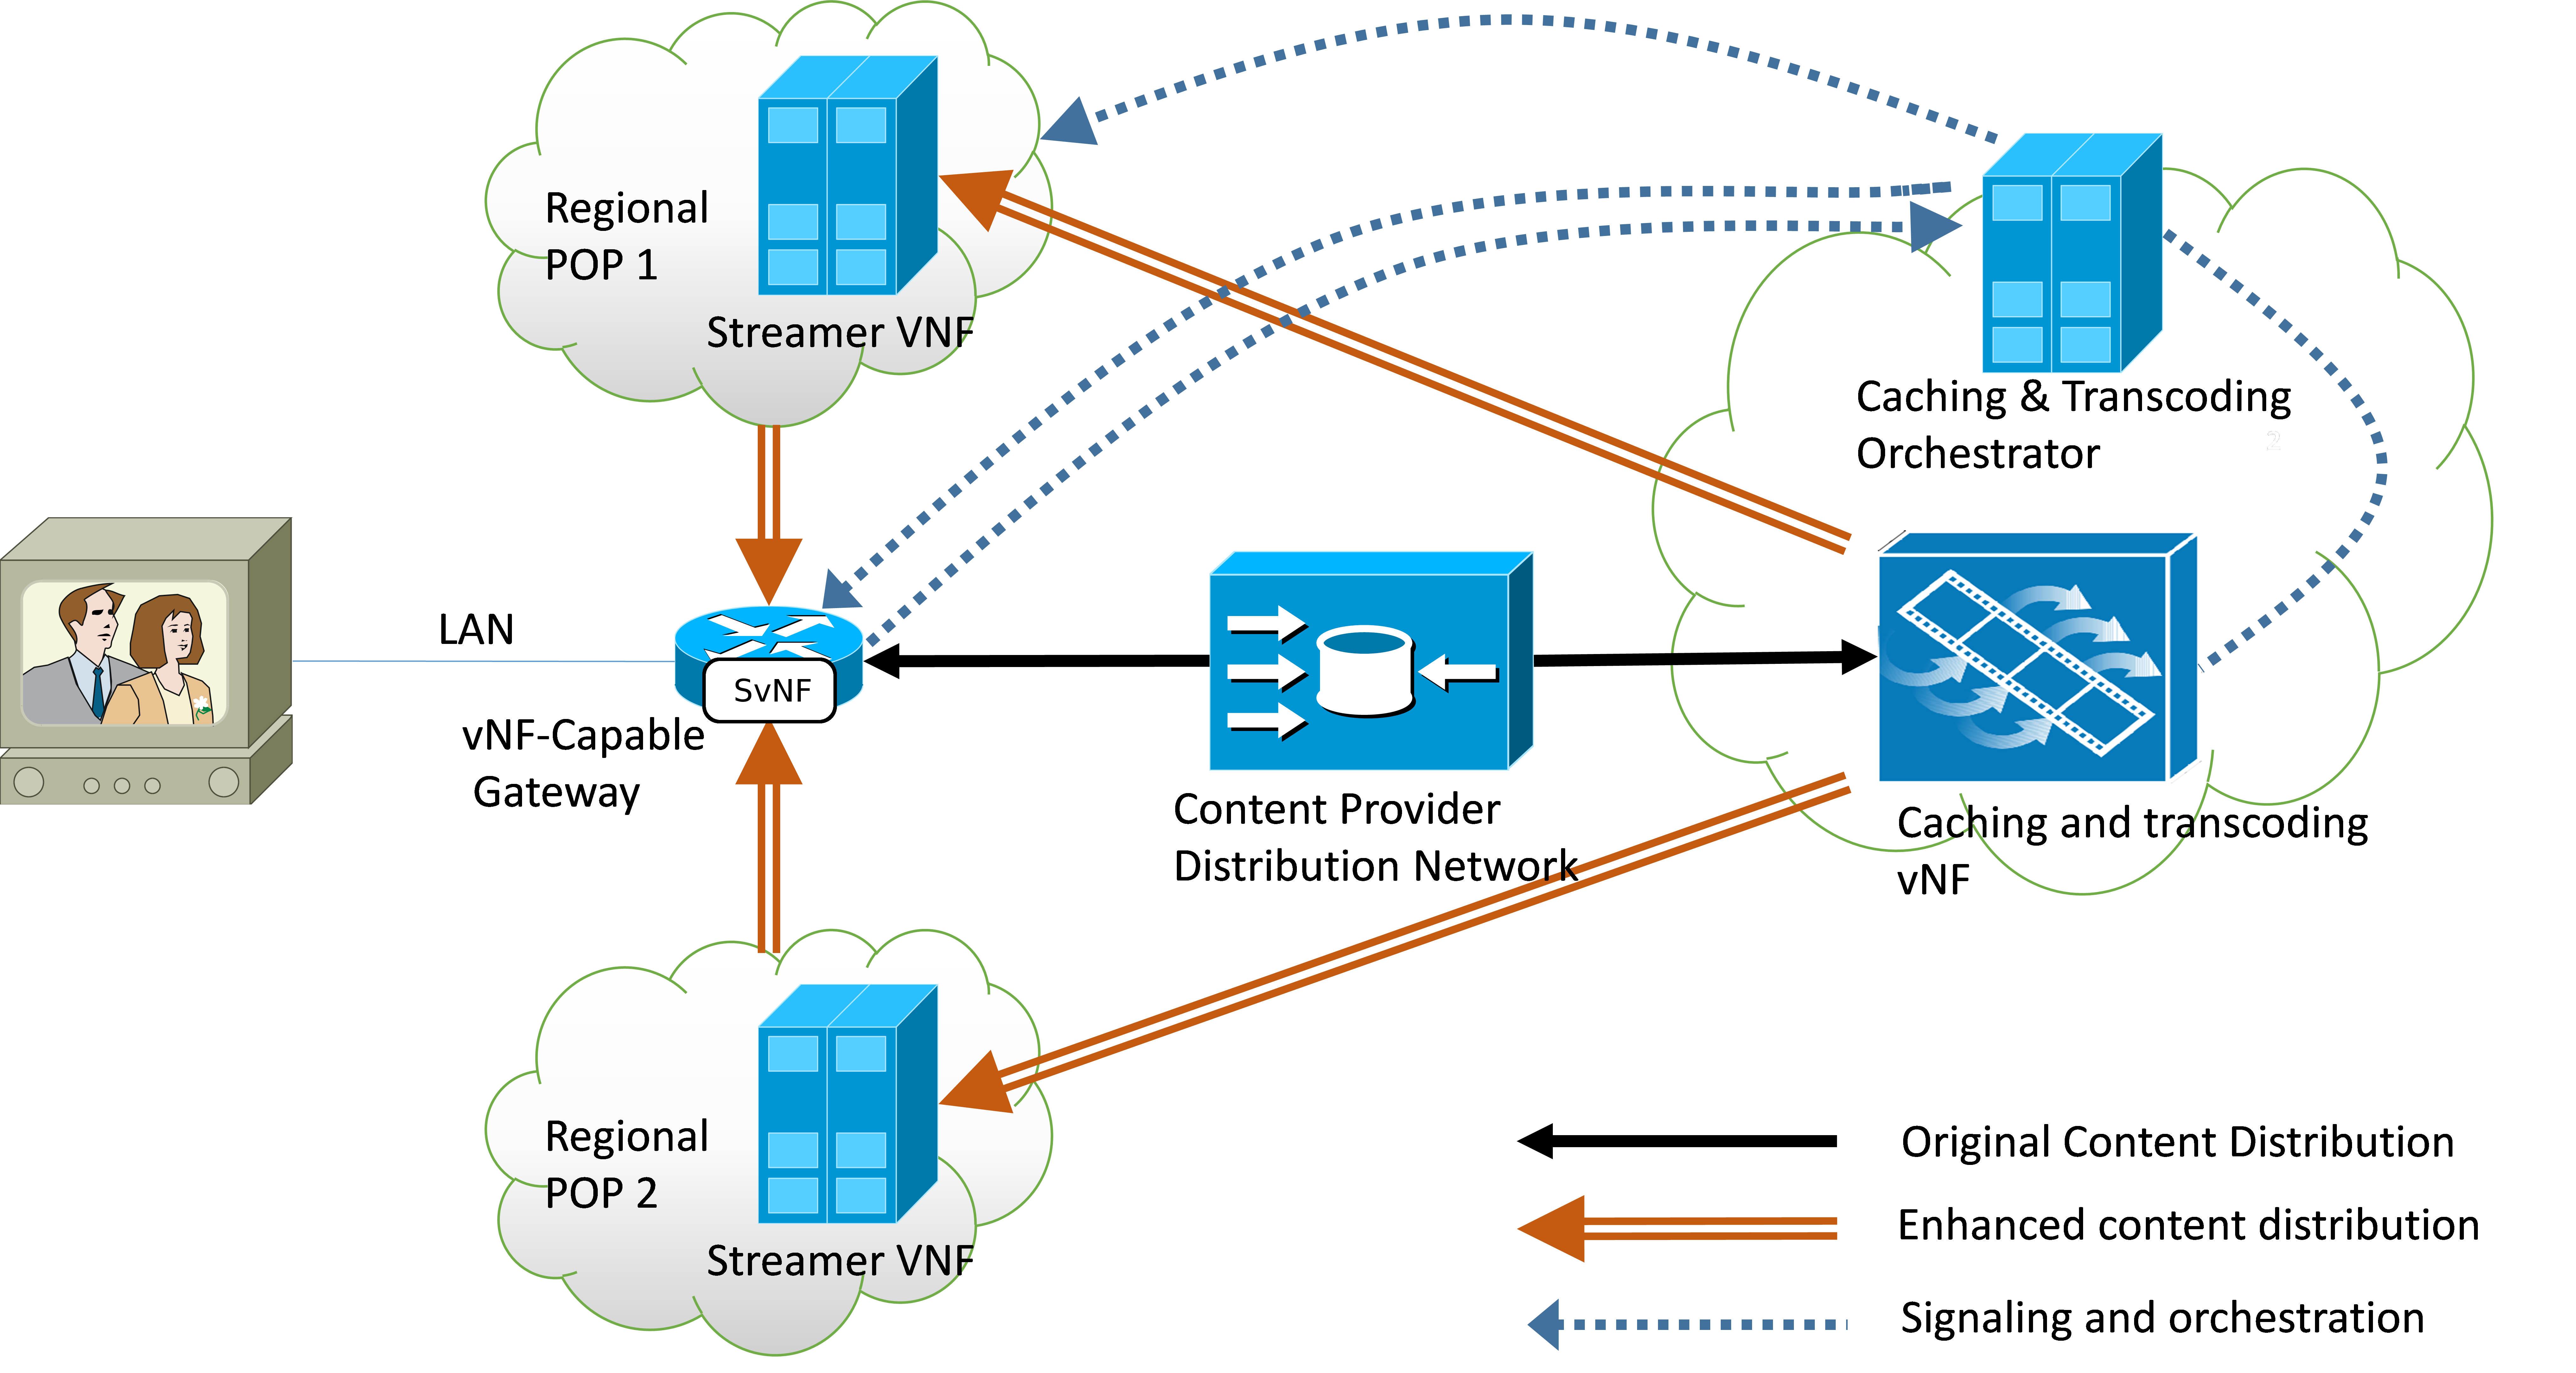
\includegraphics[width=0.90\textwidth,natwidth=8132,natheight=4335]{fig/highleveldesign.png}
	\caption{ High level design
    \label{fig:hld}
    }

\end{figure*}

The use case considered consists of an End User $u$ consuming media from his Set-Top Box, linked to his HG $G_{u}$.

Video streams of a VOD or IPTV service are transferred from the content provider distribution network \(\mathit{CP}_{\mathit{network}}\) (which may or may not include Content Delivery Networks - CDNs) to the TV and across $G_{u}$.

Figure~\ref{fig:hld} depicts the design of the system and the use case steps. The figure presents the interactions between CP, SP and EU for a classical video streaming use case.
In the original content distribution model, content is streamed from the content provider network  to the user gateway \(G_{u}\).

Classic deployment scenario involve the use of content distribution network to offload the CP main server.
CDN nodes are often collocated with internet exchange points (IXP) which present the advantage of being located relatively close of the EU.

Our use case however, presents an alternative model where the content is cached in a regional point of presence managed by the SP (also called micro-data centers located at the edge of the network). The content delivered by a streaming vNF deployed in the POP.

The caching and encoding orchestrator  $\CEO$ maintains a list of provisioned of regional POPs \(\POP=\{p_{i}\}\) that can handle cache requests. On each $p_{i}$ is deployed a set of Streaming vNF that serve content to users.

$\CEO$ also manages gateway configuration. It pushes a set of rules \(R_{u}=\{r^{u}_{1},r^{u}_{2},...,r^{u}_{n}\}\) on the $G_{u}$. 
Those rules are used to filter requests and responses crossing $G_{u}$ in order to notify the $\CEO$ that a video is requested.
It also pushes a list of cached resources available to $G_{u}$ through the POPS $C_{u}=\{c^{i,u}_{j} \}$ where $j$ is the identifier of the resource and $i$ the identifier of the POP $p_{i}$ from which it can be retreived.

The SvNF module deployed on the HG works as a HTTP proxy.
When it receives a request from client or a response from a server, it analyses it using the set of rules \(R_{u}\) and the set of cached resource $C_{u}$ deployed on the HG.
Depending on the result several scenarios can occur.
Let's consider the three possible scenarios.

%\paragraph{Step1}EU requests the content from the vNF-Capable Gateway. 
%\paragraph{Step 2}
%The vNF-Capable Gateway analyses the video format, and checks it is technically compatible with the system (e.g. a supported video codec and supported delivery method).
%If it is compatible, we continue to scenario 2, otherwise, we proceed with scenario 1.

\subsubsection*{Scenario 1: no operation scenario}

In this scenario, the content consumed by the user is not eligible to the enhancements brought by the system. None of the rules $r_{i}$ deployed on $G_{u}$ matches the request or the response and and the content doesn't match any $c^{i,u}_{j}$ either. We note $\mathbb{1}_{r_{i}}(.)$ and $\mathbb{1}_{c^{i,u}_{j}}(.)$ such that:
\[
    \mathbb{1 }_{r_{i}}(\mathit{message})= 
\begin{dcases}
    1& \text{if rule $r_{i}$ matches the message} \\
    0              & \text{otherwise}
\end{dcases}
\]
and 
\[
    \mathbb{1 }_{c^{i,u}_{j}}(\mathit{resource})= 
\begin{dcases}
    1& \text{if rule $c^{i,u}_{j}$ matches the resource} \\
    0              & \text{otherwise}
\end{dcases}
\]

After the gateway has analysed the request, it is forwarded to its original destination.

\begin{algorithmic}[1]
	
\STATE User $u$ requests a resource
\STATE $G_{u}$ receives request $\mathit{Req}$ from $u$
\STATE \( \sum_{r^{u}_{i}\in R_{u}}{\mathbb{1}_{r_{i}}(\mathit{Req})}=0 \)
\STATE \( \sum_{c^{i,u}_{j}\in C_{u}}{\mathbb{1}_{c^{i,u}_{j}}(\mathit{Req})}=0 \)
\STATE $G_{u}$ forward $\mathit{Req}$ to its original destination \(\mathit{CP}_{\mathit{network}}\)
\STATE $G_{u}$ receives response $\mathit{Res}$ from \(\mathit{CP}_{\mathit{network}}\)
\STATE \( \sum_{r^{u}_{i}\in R_{u}}{\mathbb{1}_{r_{i}}(\mathit{Res})}=0 \)
\STATE User $u$ receives $\mathit{Res}$ from \(\mathit{CP}_{\mathit{network}}\) through $G_{u}$
\end{algorithmic}


As the content is then directly consumed by the End-User from the Content Provider Delivery Network.
This is the common case, as it is performed today. The HG does not bring any added value to the consumption of video streams. It just lets the content pass through it.

In this case, the SvNF creates an overhead on the gateway without bringing additional value to the user.
This overhead needs to be measured in order to know if it would penalize the user experience (and in which extent).

\subsubsection*{Scenario 2: Cache hit scenario}

In this scenario, some resources have been retreived from \(\mathit{CP}_{\mathit{network}}\), transcoded and provisionned in a POP $p_{i}$ available to $G_{u}$.

\begin{algorithmic}[1]
	\STATE User $u$ requests a resource
\STATE $G_{u}$ receives request $\mathit{Req}$ from $u$
\STATE \( \sum_{c^{i,u}_{j}\in C_{u}}{\mathbb{1}_{c^{i,u}_{j}}(\mathit{Req})}>0\)
\STATE $G_{u}$ forward $\mathit{Req}$ selected $p_{i}$
\STATE $G_{u}$ receives response $\mathit{Res}$ from $p_{i}$
\STATE User $u$ receives $\mathit{Res}$ from $p_{i}$ through $G_{u}$
\STATE $p_{i}$ notified $\CEO$ that it served  $\mathit{Req}$
\end{algorithmic}


In this scenario, the content has been processed by the system and is made available in regional POPs.
Those are part of the NVF infrastructure, and handle storage and content delivery.
They are managed by SP and can be collocated with existing O-CDNs (operator-managed CDN).
vNFs are deployed in regional POPs and provisioned close to the user, limiting the number of hops with respect to the original Content Provider network.
As the network become capable of handling both delivery and transcoding, bandwidth and storage consumptions are reduced. Considering that orchestrator can detect which version (low, standard or high def) should be provisionned, in which POP and use just in time transcoding to generate only the version to be deployed.

\subsubsection*{Scenario 3: Cache miss scenario}

In this scenario, the resource targeted by the user matches the Rules, but is not available.

\begin{algorithmic}[1]
\STATE User $u$ requests a resource
\STATE $G_{u}$ receives request $\mathit{Req}$ from $u$
\STATE \( \sum_{c^{i,u}_{j}\in C_{u}}{\mathbb{1}_{c^{i,u}_{j}}(\mathit{Req})} = 0 \)
\STATE \( \sum_{r^{u}_{i}\in R_{u}}{\mathbb{1}_{r_{i}}(\mathit{Req})} > 0  \)
\IF { $M_{req}>0$}
\STATE $G_{u}$ informs $\CEO$ that $u$ requested $\mathit{Req}$
\ENDIF
\STATE $G_{u}$ forward $\mathit{Req}$ to its original destination \(\mathit{CP}_{\mathit{network}}\)

\STATE $G_{u}$ receives response $\mathit{Res}$ from \(\mathit{CP}_{\mathit{network}}\)
\IF { $M_{req} = 0$ }
	\STATE \( \sum_{r^{u}_{i}\in R_{u}}{\mathbb{1}_{r_{i}}(\mathit{Res})}=M_{res}\) 
	\IF { $M_{res} = 0$}
	\STATE $G_{u}$ informs $\CEO$ that $u$ received $\mathit{Res}$
	\ENDIF
\ENDIF

 
\STATE User $u$ receives $\mathit{Res}$ from \(\mathit{CP}_{\mathit{network}}\) through $G_{u}$
\end{algorithmic}

Here, $\CEO$ is informed that a cache request has not been fulfilled. According to its provisionning algorithm, it can decide to deploy the resource corresponding to $\mathit{Req}$ in a $p_{i}$ wether by transcoding the original file from \(\mathit{CP}_{\mathit{network}}\) to a $p_{i}$ or by reprovisionning $c^{k,u}_{j}$ to $p_{i}$.
 If a modification has been operated on the POPS, $\CEO$ will update the gateways cache tables.

Finally, the last scenario is the one where the content is eligible for caching and transcoding but no cached version is yet available to the vHG from where the request has been made.
In this case the cache is missed and the content is retrieved from the CP.

Caching and Transcoding Orchestrator takes the decision to perform caching and transcoding on the content based on several criteria ranging from Context and User Intelligence (which has been proven in \cite{wang_cpcdn:_2015} to improve the performance of content delivery), to business negotiation between CP and SP.

\subsection{In-network processing benefits for CP and SP}
The NFV approach allows us to process data directly in the network.
For our use case, it means that we can apply arbitrary modification to a video with a view to optimize the delivery with respect to a specific technical or business objective.
For example, targeted ads can be added to the video by the SP with a view to increase profit, QOE can be increased by transcoding the content into a specific format which has this property.
The fact that we are able to transform the content directly into the network is a big advantage in term of flexibility and convenience of administration for CP and SP.

One other striking features of NFV is its ability to dynamically provision network functions according to simple business requirements expressed as Service Layer Agreements (SLA).
To fine-tune orchestration policy of the system, SP could set a target of 10Mps in the 7pm-10pm time slot for its user toward a specific VOD website.
Once the vNF is configured with those targets, Caching and Transcoding Orchestrator has to do its best to respect the SLA by using NFV infrastructure metrics (CPU, IO, Memory) but also specific application metrics.
Thanks to the key roles played by the HG, our solution offers the possibility to collect metrics at the user level and hence using a Collective Intelligence approach to optimize system operation according to SLA targets. 

Collective intelligence data is collected thanks to caching requests emitted by vHG.
The system gathers data which reflect video consumption patterns on a per-user basis, like user average bandwidth, hourly consumption patterns, and consumption habits.
Let's imagine a particular user watch HBO's Game of Thrones every Monday evening on his Ipad which support Apple's HTTP Live Streaming (HLS) on a T1 connection.
If this pattern is widespread amongst users, the Caching and Transcoding Orchestrator can assign a higher priority on the transcoding of the HD HLS version of the popular TV show and assuring the correct provisionning on selected regional POPs.

This approach allows CP to broadcast its content in cooperation with SP NVF network with limited technical interaction.
Indeed, expressing contractual SLA target is enough for the CP to deploy its content, as the SP's vNF becomes responsible for determining (1) which content to cache (2) which enhancements to bring to the content and (3) where to cache the content.
